\documentclass[a4paper, parskip=full]{scrartcl}
\usepackage[top=3cm, bottom=3.5cm, left=3cm, right=3cm]{geometry}
\usepackage[utf8]{inputenc} % use utf8 file encoding for TeX sources
\usepackage[T1]{fontenc}    % avoid garbled Unicode text in pdf
\usepackage[german]{babel}  % german hyphenation, quotes, etc
\usepackage{graphicx}       % provides commands for including figures
\usepackage[export]{adjustbox}
\usepackage{csquotes}       % provides \enquote{} macro for "quotes"
\usepackage{hyperref}       % detailed hyperlink/pdf configuration
\usepackage{color}
\usepackage{pdflscape}
\usepackage{tcolorbox}
\usepackage{hyperref}
\usepackage{tabu}			% provides tables
\usepackage{listings}
\usepackage{xcolor}
\usepackage{colortbl}
\usepackage{pdfpages} % to insert pdf files
\usepackage[nonumberlist]{glossaries}     % provides glossary commands
\hypersetup{                % ‘texdoc hyperref‘ for options
  pdftitle={Qualitätssicherung},
  pdfauthor={Anna Csurkó, Jona Enzinger, Yannik Schmid, Jonas Zoll},
}
\graphicspath{{./figures/}} % Setting the graphicspath

\title{Qualitätssicherung}
\author{Anna Csurkó, Jona Enzinger, Yannik Schmid, Jonas Zoll}
\makeatletter

\definecolor{mintgreen}{RGB}{50,161,137} % theme color of the Karlsruhe Institute of Technology (KIT)
\colorlet{punct}{red!60!black}
\definecolor{background}{HTML}{EEEEEE}
\definecolor{delim}{RGB}{20,105,176}
\colorlet{numb}{magenta!60!black}

%environments
\newenvironment{Change}[1]{
  \subsection{#1}
  \begin{tcolorbox}[title=#1,colbacktitle=mintgreen,colframe=mintgreen,colback=white]
    }{
  \end{tcolorbox}
  }   


% header and footer
\usepackage[automark,autooneside=false,headsepline=0.5pt,footsepline=0.5pt]{scrlayer-scrpage}
\addtokomafont{headsepline}{\color{mintgreen}}
\addtokomafont{footsepline}{\color{mintgreen}}
\addtokomafont{pagehead}{\normalfont}

% delete current settings for header and footer
\clearpairofpagestyles

% display document name on the left and current section on the right
\ihead{\@title}
\ohead{\rightmark}

% load glossary entries
\makenoidxglossaries
\loadglsentries{./chapters/Glossareintraege}

% center page number
\cfoot*{\pagemark}

\setcounter{secnumdepth}{3}

\begin{document}
% beginn content
\begin{titlepage}
  \centering
  
\includegraphics[width=0.5\linewidth]{KITLogo.png}\par\vspace{1cm}
	  {\scshape \bfseries Lehrstuhl für Pervasive Computing Systems\par}
	  {\scshape \bfseries Teco\par}
	  \vspace{0.25cm}
  	{\scshape Tobias Röddiger\\Dr. Paul Tremper\par}
  	\vspace{1.5cm}

    \newcommand{\HRule}{\rule{\linewidth}{0.5mm}}
    {\color{mintgreen}\HRule} \\[0.4cm]
  	{\huge \bfseries \LARGE Anwenderorientierte Nutzerschnittstelle für Luftqualitätsdaten\par}
    {\color{mintgreen}\HRule} \\[1cm]
  	\vspace{2cm}
  	{\scshape \Large Anna Csurkó\\Jona Enzinger\\Yannik Schmid\\Jonas Zoll\par}
  	\vfill

\end{titlepage}


\tableofcontents
\section{Einleitung}







\section{Testfälle}
\subsection{Basis-Testfälle}
\begin{center}
    \begin{tabular}[h]{|c|l|c|}
        \hline
        \textbf{TF} & \textbf{Bezeichnung} & \textbf{Bestanden} \\
        \hline
        /TF10/ & Webanwendung öffnen & \cellcolor{green!25}OK \\
        \hline
        /TF20/ & Karte bewegen & \cellcolor{green!25}OK \\
        \hline
        /TF30/ & Handylayout & \cellcolor{red!25}FAILED \\
        \hline
        /TF40/ & Zoomen & \cellcolor{green!25}OK \\
        \hline
         /TF50/ & Einen Pin einer Messtation anklicken & \cellcolor{green!25}OK \\
        \hline
        /TF60/ & Karte auswählen & \cellcolor{green!25}OK \\
        \hline
        /TF70/ & Färbungsskala anzeigen & \cellcolor{green!25}OK \\
        \hline
         /TF80/ & Ort suchen & \cellcolor{green!25}OK \\
        \hline
         /TF90/ & Fehlermeldung bei der Suche & \cellcolor{red!25}FAILED \\
        \hline
        /TF100/ & Zum jetzigen Standort springen & \cellcolor{green!25}OK \\
        \hline
        /TF110/ & Scrollen & \cellcolor{green!25}OK \\
        \hline
         /TF120/ & Zeitrahmen einstellen & \cellcolor{green!25}OK \\
        \hline
         /TF130/ & Vergleich mit letztem Jahr & \cellcolor{green!25}OK \\
        \hline
         /TF140/ & Grenzwertüberschreitung & \cellcolor{red!25}FAILED \\
        \hline
        /TF150/ & Zur Karte zurückkehren & \cellcolor{green!25}OK \\
        \hline
         /TF160/ & Webanwendung schließen & \cellcolor{green!25}OK \\
        \hline

    \end{tabular}
\end{center}

\subsection{Erweiterte Testfälle}

\begin{center}
    \begin{tabular}[h]{|c|l|c|}
        /TF170/ & Ladeanzeige & \cellcolor{green!25}OK \\
        \hline
        /TF180/ & Positionsanzeige & \cellcolor{green!25}OK \\
        \hline
         /TF190/ & Sprache wechselnn & \cellcolor{green!25}OK \\
        \hline
         /TF200/ & An Städte einzoomen & \cellcolor{green!25}OK \\
        \hline
        /TF220/ & Sensorinformationen & \cellcolor{green!25}OK \\
        \hline
         /TF230/ & Polygon & \cellcolor{green!25}OK \\
        \hline
         /TF240/ & Position der Karte merken 1 & \cellcolor{green!25}OK \\
        \hline
          /TF250/ & Position der Karte merken 2 & \cellcolor{green!25}OK \\
        \hline

    \end{tabular}
\end{center}

\subsection{Stabilitättests}
  \begin{center}
      \begin{tabular}[h]{|c|l|c|}
       /TF260/ & Weit auszoomen & \cellcolor{red!25}FAILED \\
        \hline
          /TF270/ & Schnelles anfordern von Daten & \cellcolor{green!25}OK \\
        \hline
      \end{tabular}
  \end{center}

\subsection{Modifizierte Testfälle}

\begin{center}
   	\item[/TF70/ Färbungsskala anzeigen]  Kartenansicht ist offen. \\ \textbf{Erwartetes Ergebnis:} Links unten ist eine Färbungsskala zu sehen. Die Skala ändert sich beim Wechseln der Feature, aber nicht beim Zoomen.
\textbf{Änderung:} Die Skala ist immer in der rechten unteren Ecke, Anklicken ist nicht nötig und bewirkt nichts.

   	\item[/TF230/ Polygon] Der Nutzer wählt beim FeatureSelect Polygonkonfiguration aus. \\ \textbf{Erwartetes Ergebnis:} Die Pins verschwinden und die Messstaionen werden mit Linien verbunden. Die Verbindungen haben Dreieckform.
\textbf{Änderung:} Der Nutzer zieht nicht selber die Polygonen.

\item[/TF260/ Weit auszoomen] Der Nutzer zoomt so weit aus wie möglich.\\ \textbf{Erwartetes Ergebnis:} Die Karte zoomt aus und stoppt da. Beim weiten Auszoomen verschwinden die Pins, die beim Einzoomen auf ein Land/eine Ort wieder erscheinen. Keine fehlermeldung oder Absturz.
\textbf{Änderung:} Keine Polygonen sollen erscheinen. Es werden nicht mehr Daten geladen als im eingezoomten Zustand, deswegen wurde der Test umbenannt.

\subsection{Gelöschte Testfälle}

\begin{center}
   	\item[/TF210/ Durchschnitt] \textbf{Grund der Löschung:} Durch die riesige Menge an Messwerten, die die berechnung zum absturz bringen, und durch die lange Wartezeit beim Laden der Daten, die zu Timeout führt, war es nicht mehr sinnvoll dises Diagramm in die Applikation einzubauen. So gibt es bei deisem Test nichts zum Testen. 

\end{center} 


\subsection{Erweiterte Testfälle}

Keine Testfälle wurden hinzugefügt.

	






\section{Unit tests}

\subsection{Eingesetzte Software}

Für die Qualitätssicherung nutzen wir schon seit der Implementierungsphase Jest, um die Funktionalitätr der einzelnen methoden zu teste. Das haben wir zusätzlich mit enzyme ergänzt, womit wir die Funktion gesamter React-Komponenten einfach testen können.

\subsection{Testcoverage}
\includegraphics[width=1\linewidth]{figures/Testcoverage-vorläufig1.png}\par\vspace{1cm}
\includegraphics[width=1\linewidth]{figures/Testcoverage-vorläufig2.png}\par\vspace{1cm}

\subsection{Bugs and Fixes}

\subsubsection{Karte auszoomen}
\paragraph{Problem}
Wenn die größtmöglichen Koordinaten erreicht werden, die Webanwendung stürzt ab.

\paragraph{Lösung}
Wir haben eine Grenze für das maximale Auszoomen gesetzt. So passt nur ca. europa frauf aber man kann die Karte weiterschieben.



\section{Usability Test}
Bei den Usability Tests wird das fertige Produkt an echten Testpersonen getestet, deren  Meinungen und Reaktionen erfasst und analysiert werden. Dadurch wird die Benutzerfreundlichkeit und intuitive Bedienenug des Produktes gemessen. Diese Test sind essenziell, da das Entwicklerteam, das schon von anfang an an das Projekt arbeitet die Funktionalität des Programms vollständig kennt und deshalb die Intuitivität (Bedienung ohne jegliche Kenntnis des Programms) nicht beurteilen kann.

  \subsection{Testpersonen}
    Die Testpersonen sind - wie unsere Zielgruppe - eher älter, wobei keine genaue untere Grenze gesetzt ist und die Meinungen der Testpersonen außerhalb unserer Zielgruppe gleich wertvoll für uns sind. Es ist wichtig, dass die Testsubjekte über wenig bis gar kein Wissen über Feinstaubindex bzw. Luftqualität verfügen, da die Applikation insbesondere für solche Menschen entwickelt wurde. Personen, die wenig über Softwareentwicklung wissen, werden bevorzugt. Die Testsubjekte hauptsächlich Bekannten des Entwicklerteams, da die Applikation nicht als Webseite zugänglich ist und weil für den Test die Beobachtung, Erklärung und Fragestellung eines Teammitglieds mit breitem Wissen über die Applikation wichtig ist.

  \subsection{Testmethode}
    Um ein umfassendes Bild über die Usability unserer Webanwendung zu bekommen haben wir einen umfangreichen Usability-Test entworfen. Der Test besteht im wesentlichen aus 3 Teilen, die im folgenden noch genauer beschrieben werden. Den kompletten Test finden Sie im Anhang.
    Wir haben den Test mit jeder Testperson einzeln, an verschiedenen Geräten (PC/Laptop/Tablet/Smartphone) durchgeführt.

    \subsubsection*{System Usability Scale}
      Durch die System Usability Scale wird die subjektiv wahrgenommene Gebrauchstauglichkeit des Programs bewertet. Die Testsubjekte müssen zehn Fragen mit Werten von 1 bis 5 bewerten. Bei der System Usability Scale handelt es sich um einen standartisierten Fragebogen, der es erlaubt die Qualität einer Benutzeroberfläche in Zahlen auszudrücken und somit vergleichbar zu machen.
      
    \subsubsection*{Think Aloud}
      Beim Teil 'Think Aloud' des Usability Tests wurden den Testpersonen einfache Frage und Aufgaben gestellt. Die Tester wurden angewießen die die Fragen intuitiv zu beantworten, beim Lösen der Aufgaben pragmatisch vorzugehen und ihre Gedankengänge dabei laut auszusprechen.
    
    \subsubsection*{Erweitereter Fragebogen}
      Hier haben wir vor allem Freitext-Fragen abgefragt, unter anderem die Frage, was den Testpersonen am meisten/wenigsten an der Webanwendung gefallen hat und welche Optimierungen sie uns empfehlen würden.

  \subsection{Auswertung}
    Da die Antworten unserer Testpersonen sehr umfangreich und teilweise auch sehr unterschiedlich waren, haben wir uns im folgenden auf eine Zusammenfassung der relevanten Erkenntnisse beschränkt.

    \subsubsection{Think Aloud}
      \paragraph{Kartenansicht}
        Der erste Eindruck der Tester zur Kartenansicht war in 90\% der Fälle positiv. Viele erwähnten, dass sie das Design übersichtlich und intuitiv fänden. Zwei Tester zogen einen Vergleich zu anderen Kartenanwendungen.

        Anschließend haben wir einige Aufgaben gestellt, um zu sehen, wie die Tester intuitiv vorgehen, um verschiedene Orte auf der Karte zu finden. Hierbei viel auf, dass hauptsächlich die Suchfunktion genutzt wurde. Die anderen Tester zoomten heraus, verschoben die Karte und zoomten an der gewünschten Stelle wieder herein.

        Anschließend versuchten wir mit einigen Fragen herauszufinden, ob die Darstellung der Messstationen als Marker auf der Karte intuitiv ist. Alle Tester bestätigten das. Spätestens nach dem anklicken eines Markers nannten alle Tester die richtige Bedeutung der Marker und der dargestellten Daten.

        Die nächsten Aufgaben zielten darauf ab, die Benutzbarkeit der Kartenkonfiguration zu testen. Die Tester wurden angewießen verschiedene Information in der Webapp zu finden. Unter anderem sollte der Temparatur Höchstwert innerhalb Augsburg ermittelt werden. Mit der Standarteinstellung war das zwar möglich, aber sehr umständlich, da bei ähnlichen Temparaturen die Marker ähnlich eingefärbt waren, war das Erkennen von Unterschieden erschwerte.
        Einfacher hätte man die Aufgabe durch eine Umstellung der Karteneinstellung 'Style' lösen gekonnt, woraufhin die Messwerte nicht mehr auf einer absoluten Skala eingefärbt gewesen wären, sondern im Vergleich zu den umliegenden Stationen. Diese Einstellung wurden aber von keiner der Tester vorgenommen. Auf Nachfrage wurde angegeben, das der Begriff 'Style' in diesem Zusammenhang missverständlich sei.
     
      \paragraph{Detailansicht}
        Der erste Eindruck der Detailansicht war in allen Fällen positiv. Auch hier wurde der Aufbau der Seite als übersichtlich und schlicht beschrieben.
        Die Bedeutung des Diagramms, das die zeitliche Veränderung der Messwerte eines \glspl{Feature} anzeigt war allen Testpersonen intuitiv klar. Im Gegensatz dazu, war die Bedeutung des Tortendiagramms einigen Testpersonen unklar.
        
        Die Konfiguration der Diagramme war für alle Testpersonen intuitiv möglich.
     
    \subsubsection{Auswertung System Usability Scale}
      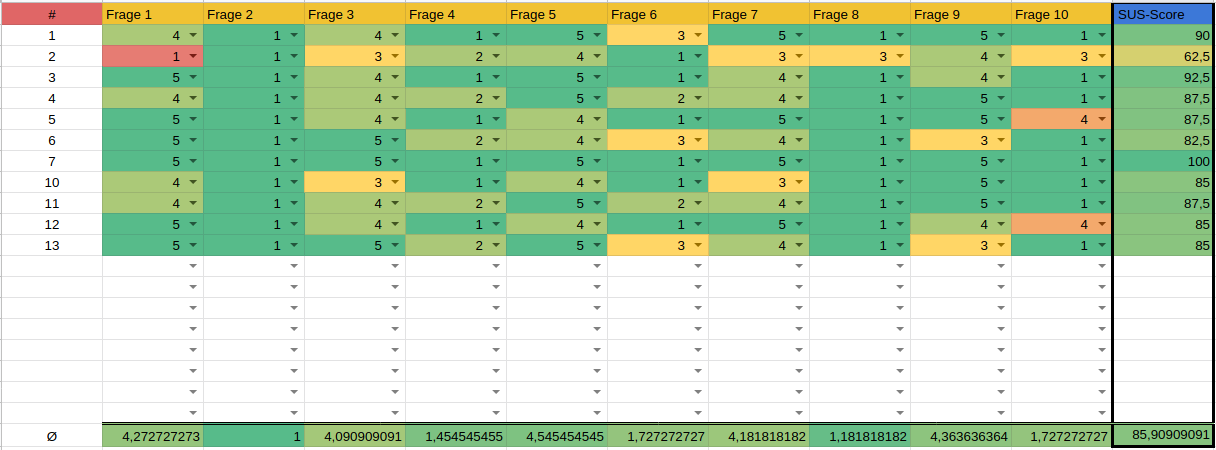
\includegraphics[width=1\linewidth]{figures/sus.png}\par\vspace{1cm}

    \subsubsection{Auswertung Erweiterter Fragebogen}
      \paragraph{Positives}
        Mehrmals wurde hier das schlichte Design der Webanwendung angegeben, das viele Tester als übersichtlich und intuitiv beschrieben haben.
        Des Weiteren wurde gelobt, dass die Webanwendung viele nützliche Informationen bereit stelle und auch Detailinformationen erreichbar seien.
        Einige Tester lobten die Einordung der Messwerte mit hilfe der Farbskala.
     
      \paragraph{Negatives und Verbesserungsvorschläge}
        Bei der Frage, welche Punkte den Testpersonen nicht an unserer Webanwendung gafallen haben, gab es bis auf einen Punkt keinen eindeutigen Trend, da die Anworten sehr unterschiedlich waren.
        Ein Tester beschrieb die Webanwendung als 'zu schlicht' und hätte sich ein auffallenderes Design und eine andere Hauptfarbe gewünscht.
        Zwei Tester bemängelten, dass nur Messstationen in Augsburg unterstützt würden.
        Ein weiterer Tester gab an, die Farben der Farbskala der Kartenansicht seien zu änlich, wodurch die Unterschiede zwischen den Messwerten unterschiedlicher Messstationen auf der Karte nur sehr schwer zu erkennen seien.
        
        Der Punkt, in dem sich die meisten Tester einig waren, war der, das die Erklärungen der Fachbegriffe (vor allem PM10 und PM2.5) nur schwer in der Webapp zu finden seien. Diese Hilfe-Funktion solle auffallender in der Webapp positioniert werden.

  \subsection{Gelöste Probleme}

    \begin{Bug}{Konfigurationsnamen}
      \textbf{Problem}\\
      Bei der Auswahl der Konfiguration wird nur der interne Name angezeigt (z.B. PolygonConfiguration),
      was wenig aussagekräftig ist. Zudem sind diese Namen nicht lokalisiert.\\
      \linebreak
      \textbf{Lösung}\\
      Die IDs der Konfigurationen bekommen einen Eintrag in der Sprachdatei um leicht verständliche
      Namen in der gewählen Sprache anzuzeigen.\\
    \end{Bug}

    \begin{Bug}{Weitere Optimierung der Detailseite für Mobilgeräte}
      \textbf{Symptom}\\
      Auf Mobilgeräten mit besonders kleinen Bildschirmgrößen sind die Diagramme der Detailseite zu klein um Details zu erkennen.\\
      \linebreak
      \textbf{Grund}\\
      Bislang gab es noch kein optimiertes Design dieser Seite für kleine Mobilgeräte.\\
      \linebreak
      \textbf{Lösung}\\
      Die Breakpoints des Grid Layouts wurden angepasst, sodass die Diagramm auf Mobilgeräten nun untereinander, anstatt in Zweierreihen angezeigt werden.\\
    \end{Bug}
      
    \begin{Bug}{FeautureSelect-Button}
      \textbf{Symptom}\\
      Das FeatureSelect-Button ist für Personen, die die Webanwendung zum ersten Mal benutzen, schwer zu finden.\\
      \linebreak
      \textbf{Grund}\\
      Das Button ist zu klein, lässt sich schwer vom Hintergrund unterscheiden. Man hat auch keine Information was es macht bis man draufklickt.\\
      \linebreak
      \textbf{Lösung}\\
      Das FeatureSelect-Menü ist bei Laden der Seite geöffnet und somit für Benutzer leicht zu finden.\\
    \end{Bug}

    \begin{Bug}{Skala}
      \textbf{Symptom}\\
      Größter Wert der Skala ist unrealistisch groß und damit ist die ganze Skala nutzlos.\\
      \linebreak
      \textbf{Grund}\\
      Die Skala ist auf den extremen Messwerten aller Messstation festgelegt. Da eine Messstation falsche Werte sendet, wird die Skala falsch eingestellt.\\
      \linebreak
      \textbf{Lösung}\\
      Entsprechende Station aus den Anfragen entfernen.\\
    \end{Bug}
      
    \begin{Bug}{Suche}
      \textbf{Symptom}\\
      Der Platzhaltersatz bei der Suche ist nicht vollständig lesbar.\\
      \linebreak
      \textbf{Grund}\\
      Feld  ist zu kurz.\\
      \linebreak
      \textbf{Lösung}\\
      Kürzerer Platzhaltertext. Die Größe des Feldes ist für normaler Städtenamen mehr als ausreichend.\\
    \end{Bug}
      
    \begin{Bug}{Vergleich mit letztem Jahr}
      \textbf{Symptom}\\
      Diagramm enthält überhaupt keine Information, was es zeigen will. Der Nutzer kann das Diagramm ohne Erklärung der Entwickler nicht verstehen.\\
      \linebreak
      \textbf{Grund}\\
      Überschrift und Beschriftung der Achsen fehlen.\\
      \linebreak
      \textbf{Lösung}\\
      Überschrift und Erklärung für Diagramme hinzugefügt.\\
    \end{Bug}

    \begin{Bug}{Polygon}
      \textbf{Symptom}\\
      Man sieht zwar die Färbung der Polygonen, aber man kann ihnen keinen Wert zuordnen.\\
      \linebreak
      \textbf{Grund}\\
      Durchschnittswert der Polygonen wird nirgendwo angezeigt.\\
      \linebreak
      \textbf{Lösung}\\
      Der Durchschnittswert wird in einem Tooltip angezeigt. Dafür musste die Polygonklasse geringfügig
      angepasst werden. Sie verwendet nun Observations statt Stations, was eine sinnvolle Erweiterung für die Zukunft ist.\\
    \end{Bug}

    \begin{Bug}{Namen der Stationen}
      \textbf{Symptom}\\
      Namen und Koordinaten der Stationen sind für die Meisten uninteressant und nichtssagend.\\
      \linebreak
      \textbf{Lösung}\\
      Zusätzlich zu den Koordinaten und dem Stationnamen haben wurde auch noch die Straße hinzugefügt.\\
    \end{Bug}

    \begin{Bug}{Fragezeichen nur auf in der Kartenansicht}
      \textbf{Symptom}\\
      Bei den Stationen-PopUps gibt es ein Fragezeichen-Button, die auf eine Webseite mit mehr Informationen über die ausgewählten Features weiterführt. Es wäre praktisch, diesr Fragezeichen auch auf der detailseite zu haben, insbesondere weil dort alle Features nebeneinander stehen und so man sich alle nacheinender anschauen kann.\\
      \linebreak
      \textbf{Lösung}\\
      Fragezeichen-Button mit gleicher Funktion zu jedem angezeigten Feature auf der Detailseite wurde hinzugefügt.\\
    \end{Bug}
    
    \begin{Bug}{Weitere Informationen - Größe und Stelle der Fragezeichen}
      \textbf{Symptom}\\
      Einige Testsubjekte fanden das Fragezeichen einfach zu übersehen und dessen Stelle unpraktisch. Nach mehr Testdurchläufen mit neuen Testsubjekten haben wir festgestellt, dass nur ein kleiner Teil der Testsubjekten das Fragezeichen problematisch gefunden hat. Einige wurden sogar extra von uns darauf angesprochen, ihre Meinung zum Fragezeichen-Button uns mitzuteilen. Sie hatten entweder keine Meinung dazu oder fanden es sogar gut.\\
      \linebreak
      \textbf{Lösung}\\
      Wir haben eine Anleitung zur Webseite hinzugefügt, und deren Button an eine auffällige Stelle platziert. In der Anleitung gibt es auch einen Kapitel über das Fragezeichen-Button mit Illustration. \\
    \end{Bug}

    \subsection{Unwichtige\textbackslash Unlösbare Probleme}

      In diesem Kapitel listen wir die Probleme auf, die wie versucht haben zu lösen, aber die Lösung wäre entweder zu aufwendig gewesen oder hätte nicht in unseren Zeitplan gepasst.

    \begin{Bug}{Sichtbarkeit der Stadtname}
      \textbf{Symptom}\\
      Die Pins bedecken den Stadtnamen. Er ist bei vielen Pins nicht mehr lesbar.\\
      \linebreak
      \textbf{Grund}\\
      Ortbeschriftungen befinden sich auf der Ebene unter den Pins.\\
      \linebreak
      \textbf{Lösung}\\
      Die Ortsnamen sind direkt in die Kachelbilder eingetragen was es unmöglich macht sie 
      auf eine andere Ebene zu verschieben. Eine Option wäre Reverse Geocoding.\\
    \end{Bug}
\section{Statistiken}

\subsection{Testcoverage}

\includegraphics[width=1\linewidth]{figures/Testcoverage-vorläufig1.png}\par\vspace{1cm}
\includegraphics[width=1\linewidth]{figures/Testcoverage-vorläufig2.png}\par\vspace{1cm}
\section{Anhang}
\subsection{Usability Test}
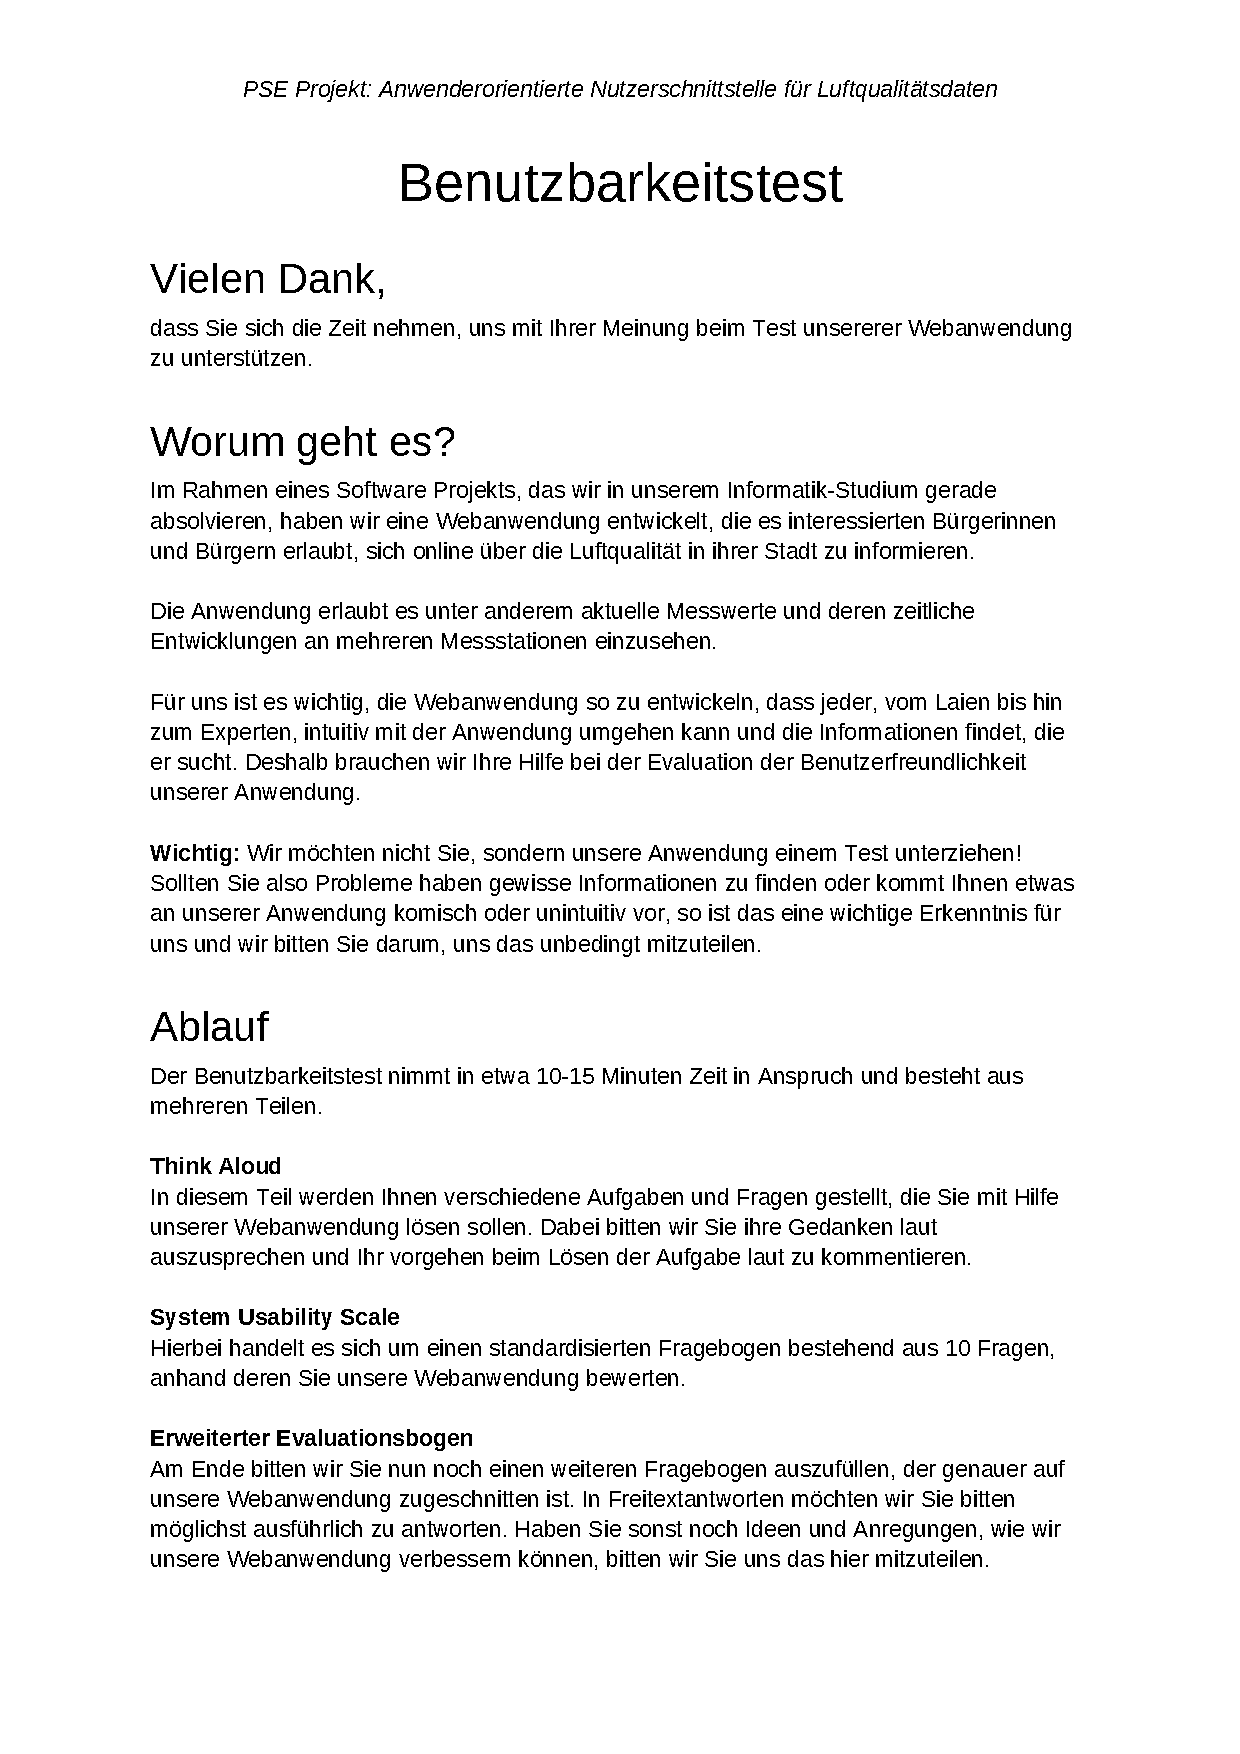
\includepdf[page=-]{./figures/usability_test.pdf}
\section{Glossar}

% automatically created glossary (compile twice to show glossary)
\glsaddall
\printnoidxglossaries


% end content
\end{document}
